\section{Durchführung}
\label{sec:Durchführung}
Zur Durchführung dieses Versuches wird der in \autoref{fig:Aufbau} gezeigte Versuchsaufbau verwendet. Im wesentlichen besteht dieser aus einem radioaktiven Präparat
($\beta$- oder $\gamma$-Strahler), einer Halterung der Absorberplatten und einem Geiger-Müller-Zählrohr (\textit{GMZ}). Es können Absorberplatten verschiedener Materialien und verschiedener
Dicke installiert werden.
Die emittierte Strahlung durchläuft die Absorbermaterialien und wird anschließend (sofern sie nicht vollständig absorbiert wurde) im Geiger-Müller-Zählrohr detektiert. 
Die Zählraten des \textit{GMZ} können über einen zuvor eingestellten Zeitbereich ermittelt und an einer digitalen Anzeige abgelesen werden.

\begin{figure}
    \centering
    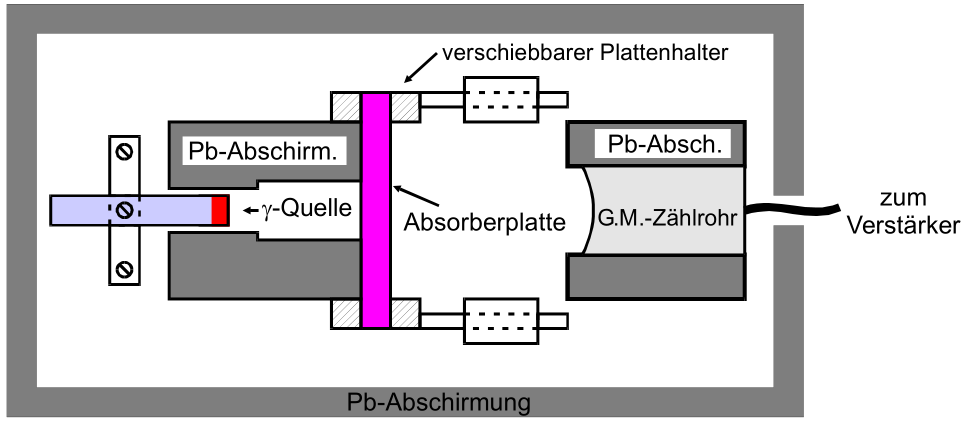
\includegraphics[width = .7\textwidth]{content/Aufbau.png}
    \caption{Aufbau des Versuches \cite{v704}.}
    \label{fig:Aufbau}
\end{figure}

Vor Beginn der eigentlichen Messreihen werden die Zählraten des \textit{GMZ} ohne Strahlungsquelle über eine Dauer von $\qty{900}{\second}$ gemessen. 
Des Weiteren wird die Zählrate des Zählrohres mit Strahlungsquelle, jedoch ohne Absorbermaterial über ein kurzes Zeitintervall gemessen.

\subsection{Messung der Absorptionskurven eines Gamma-Strahlers}
\label{subsec:D_gamma}
Zuerst wird das Absorptionsverhalten eines $\gamma$-Strahlers untersucht. Es wird Cäsium-137 als Strahlungsquelle verwendet. Für Absorberplatten aus Blei (Pb) und ein weiteres
Absorbermaterial (Eisen, Zink oder Kupfer), werden die Zählraten des \textit{GMZ} in einem Zeitbereich von $\num{100}$ bis $\qty{200}{\second}$ gemessen. Es werden 
$10$ Messwerte zu verschiedenen Dicken des Absorbers aufgenommen. Die Dicke des Absorbers lässt sich durch Kombination verschieden dicker Platten des jeweiligen Materials
variieren. Bei niedrigeren Zählraten (dickere Absorberschicht) sollte ein größeres Intervall der Messzeit gewählt werden. Es werden jeweils Dicke der Absorberschicht,
die Zählraten des \textit{GMZ} und die Zählzeit notiert. 
Aus den Messwerten kann mittels Ausgleichsrechnung der Absorptionskoeffizient des verwendeten Absorbermaterials bestimmt werden.

\subsection{Messung der Aluminium-Absorptionskurve eines Beta-Strahlers}
Im zweiten Teil des Versuches wird die Absorptionskurve von Technezium-99 bei Verwendung eines Aluminiumabsorbers ausgewertet. Auch hier werden zu verschiedenen Dicken 
der Absorberschicht die Zählraten des \textit{GMZ} gemessen. Es sollten Zeitintervalle von $200$ bis $\qty{400}{\second}$ betrachtet werden, wobei zu größeren Dicken der
Absorberschicht wieder ein größeres Zeitintervall gewählt werden sollte.
Aus den Messwerten lässt sich die maximale Energie des $\beta$-Strahlers ermitteln.
